\subsection{Performance Requirements}
\begin{itemize}
	\item Reliability: The correct algorithms, datasets and experiments should be returned when requested. \newline
    \item Data Integrity: Consistent, correct and complete output should always be generated for all supported input to the Execution Manager and the Metrologist UI. \newline
\end{itemize}
\subsection{Design Constraints}
\begin{enumerate}
	\item The algorithms, datasets and experiments stored in the database for a specific user should be available to the input unit.
	\item The input unit should be able to communicate with the execution manager and the Metrologist UI efficiently and whenever it needs to. 
\end{enumerate}
\subsection{Software System Attributes}
\begin{flushleft}
    \par\textbf{Extensibility}: More future features and objects can be added to the input unit seamlessly without affecting the functionality of the code because the client and the underlying structure of the Experiment object have been decoupled.\newline
    
    \par\textbf{Modifiability: } The Builder design pattern enables the input unit to be highly customizable without affecting the client and other functionalities that depend on it negatively. As a result, the individual objects such as Algorithm and Datasets can be accessed independently or combined to form a more complex Experiment object without affecting the client's usage.\newline
  
    \par\textbf{Robustness}: Object modification an side-effect generations are minimized which ensures that few code failures are generated. \newline
    
    \par\textbf{Availability}: Objects generated will always be available to the Execution manager and the Metrologist UI on request. \newline
    \end{flushleft}

\subsection{Class diagram}
	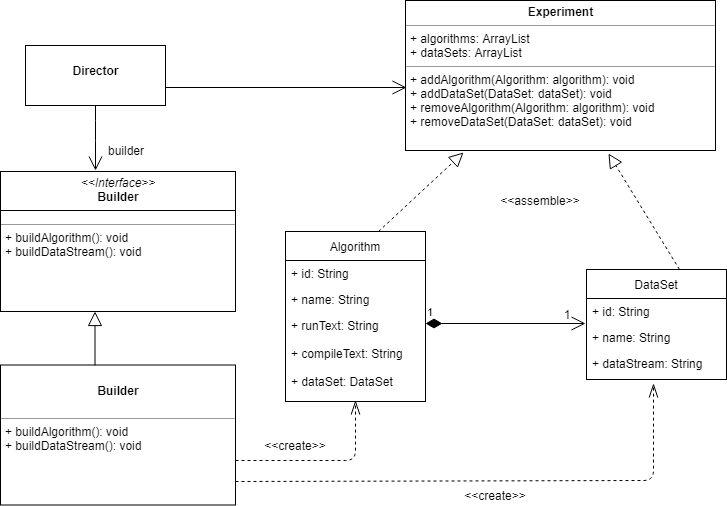
\includegraphics[width=12cm,height=15cm,keepaspectratio]{input_unit/images/input_unit_class_diagram.png}
	\begin{center}
	    \small{Figure 11: Class diagram for Input Unit}
    \end{center}
 \begin{flushleft}
\par\textbf{Design Pattern Used: }
	I used the Builder design pattern because it enables the Algorithm and DataSet objects to be configurable so that multiple types of data sets, compilation environments and executables can be considered with minimal effort to the developer. The consumer of the service has no access to the underlying structure of the object requested and so decoupling is highly utilized. This also allows the client to directly instantiate the Algorithm and DataSet classes as self-standing objects that can be used for other purposes.
    \end{flushleft}
	\newpage
\subsection{Activity diagrams for Input Unit}
	\subsubsection{Create Algorithm}
    \par With regards to Experiment and Data sets,
{ \textit{mutatis muntandis} the same as regarding algorithms.} \newline \newline
    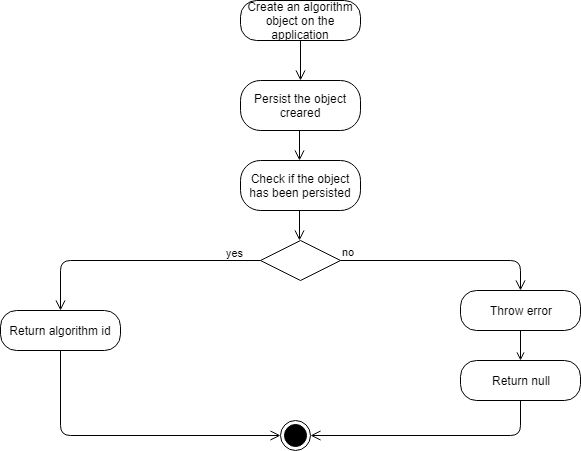
\includegraphics[width=12cm,height=15cm,keepaspectratio]{input_unit/images/create_algorithm_activity_diagram.png}
	\begin{center}
	    \small{Figure 12: Activity diagram for Creating an algorithm }
    \end{center}
    \newpage
    \subsubsection{Remove Algorithm}
    \par With regards to Experiment and Data sets,
{ \textit{mutatis muntandis} the same as regarding algorithms.} \newline \newline
    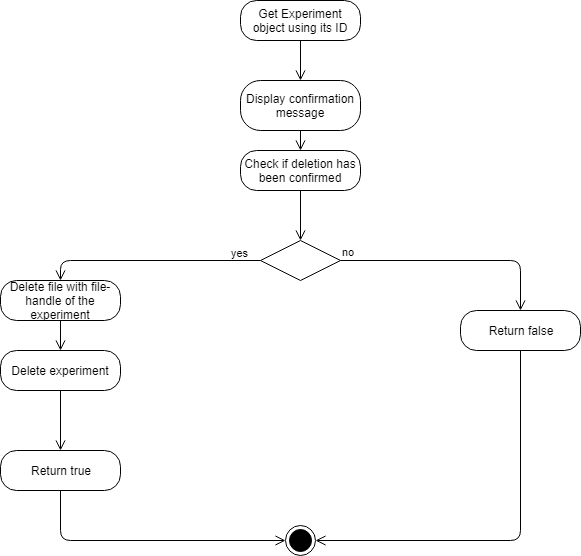
\includegraphics[width=12cm,height=15cm,keepaspectratio]{input_unit/images/delete_activity_diagram.png}
	\begin{center}
	    \small{Figure 13: Activity diagram for Deleting an algorithm }
    \end{center}
    \newpage
    \subsubsection{Get Algorithm}
    \par With regards to Experiment and Data sets,
{ \textit{mutatis muntandis} the same as regarding algorithms.} \newline \newline
    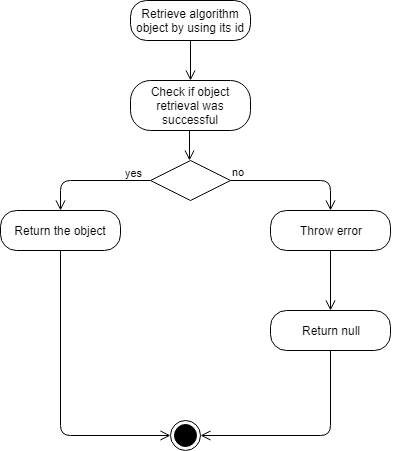
\includegraphics[width=12cm,height=15cm,keepaspectratio]{input_unit/images/get_algorithm_activity_diagram.png}
	\begin{center}
	    \small{Figure 14: Activity diagram for getting an algorithm }
    \end{center}
    \newpage
    \subsubsection{Update An Algorithm's Name}
    \par With regards to Experiment and Data sets attributes, as well as other algorithm's attributes,
{\textit{mutatis muntandis} the same as regarding an update to an algorithm's name.} \newline \newline
    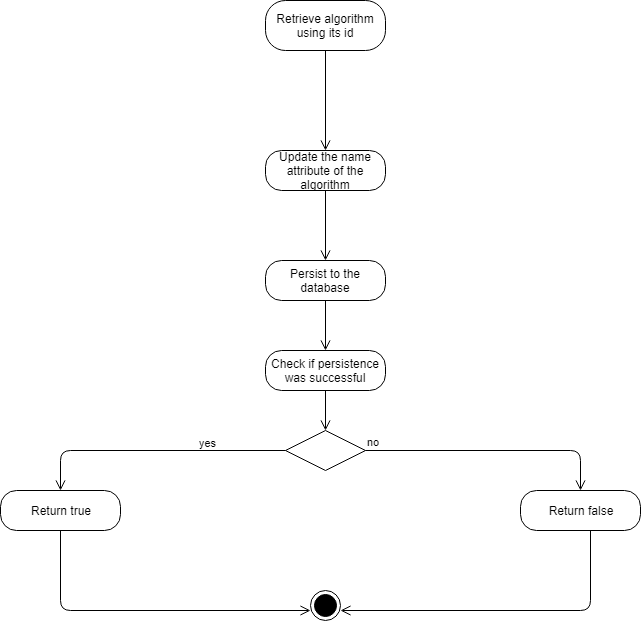
\includegraphics[width=12cm,height=15cm,keepaspectratio]{input_unit/images/update_algorithm_activity_diagram.png}
	\begin{center}
	    \small{Figure 15: Activity diagram for updating an algorithm's name attribute }
    \end{center}
	\newpage

\subsection{Sequence diagrams for Input Unit}
	\par{Please note that a "service consumer" is a general term to group the Execution Manager and Metrologist UI consumers that use the Input Unit.}
    	\subsubsection{Create Algorithm}
    \par With regards to Experiment and Data sets,
    {\textit{mutatis muntandis} the same as regarding algorithms.} \newline \newline
    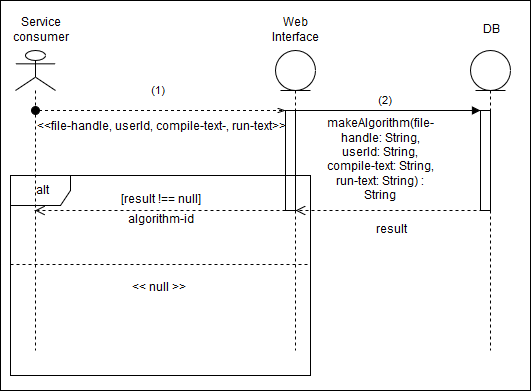
\includegraphics[width=12cm,height=15cm,keepaspectratio]{input_unit/images/create_algorithm_sequence_diagram.png}
    \begin{center}
    	\small{Figure 16: Sequence diagram for Creating an algorithm }
    \end{center}
    \newpage
    \subsubsection{Remove Algorithm}
    \par With regards to Experiment and Data sets,
    { \textit{mutatis muntandis} the same as regarding algorithms.} \newline \newline
    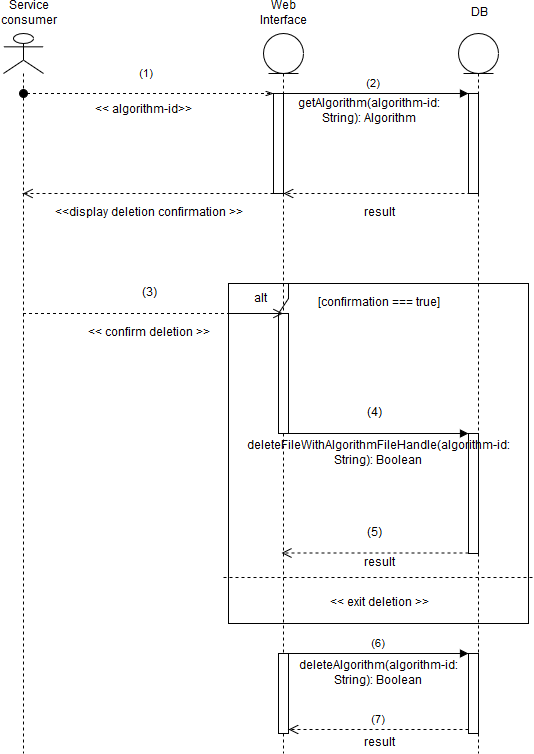
\includegraphics[width=12cm,height=15cm,keepaspectratio]{input_unit/images/delete_algorithm_sequence_diagram.png}
    \begin{center}
    	\small{Figure 17: Sequence diagram for Deleting an algorithm }
    \end{center}
    \newpage
    \subsubsection{Get Algorithm}
    \par With regards to Experiment and Data sets,
    { \textit{mutatis muntandis} the same as regarding algorithms.} \newline \newline
    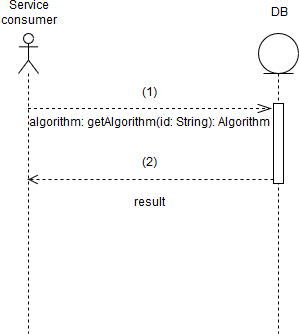
\includegraphics[width=12cm,height=15cm,keepaspectratio]{input_unit/images/get_algorithm_sequence_diagram.png}
    \begin{center}
    	\small{Figure 18: Sequence diagram for getting an algorithm }
    \end{center}
    \newpage
    \subsubsection{Update An Algorithm's Name}
    \par With regards to Experiment and Data sets attributes, as well as other algorithm's attributes,
    { \textit{mutatis muntandis} the same as regarding an update to an algorithm's name.} \newline \newline
    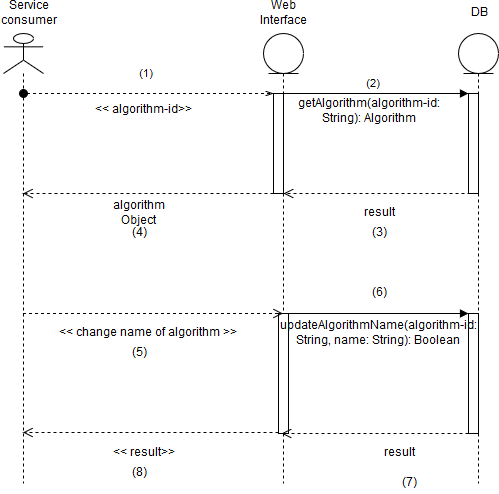
\includegraphics[width=12cm,height=15cm,keepaspectratio]{input_unit/images/update_algorithm_sequence_diagram.png}
    \begin{center}
    	\small{Figure 19: Sequence diagram for updating an algorithm's name attribute }
    \end{center}
    \newpage

\subsection{State diagrams for Input Unit}
    	\subsubsection{Create Algorithm}
    \par With regards to Experiment and Data sets,
    {\textit{mutatis muntandis} the same as regarding algorithms.} \newline \newline
    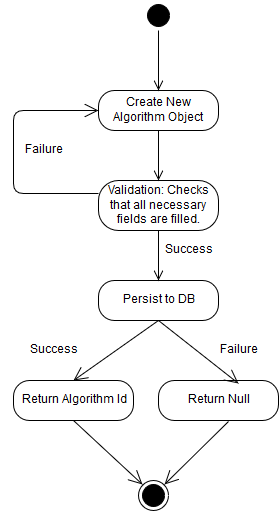
\includegraphics[width=12cm,height=15cm,keepaspectratio]{input_unit/images/create_algorithm_state_diagram.png}
    \begin{center}
    	\small{Figure 20: State diagram for Creating an algorithm }
    \end{center}
    \newpage
    \subsubsection{Remove Algorithm}
    \par With regards to Experiment and Data sets,
    { \textit{mutatis muntandis} the same as regarding algorithms.} \newline \newline
    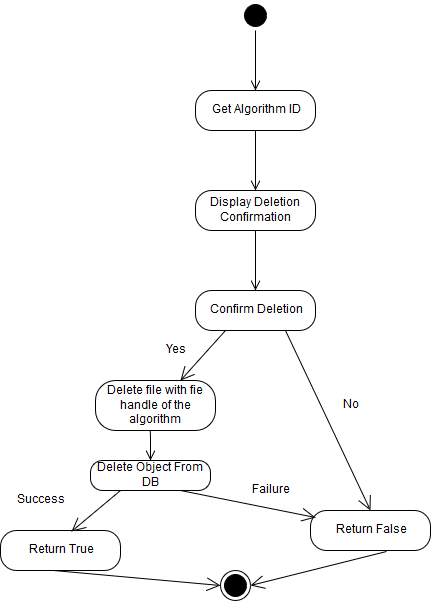
\includegraphics[width=12cm,height=15cm,keepaspectratio]{input_unit/images/delete_algorithm_state_diagram.png}
    \begin{center}
    	\small{Figure 21: State diagram for Deleting an algorithm }
    \end{center}
    \newpage
    \subsubsection{Get Algorithm}
    \par With regards to Experiment and Data sets,
    { \textit{mutatis muntandis} the same as regarding algorithms.} \newline \newline
    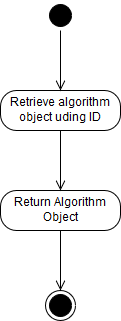
\includegraphics[width=12cm,height=15cm,keepaspectratio]{input_unit/images/get_algorithm_state_diagram.png}
    \begin{center}
    	\small{Figure 22: State diagram for getting an algorithm }
    \end{center}
    \newpage
    \subsubsection{Update An Algorithm's Name}
    \par With regards to Experiment and Data sets attributes, as well as other algorithm's attributes,
    { \textit{mutatis muntandis} the same as regarding an update to an algorithm's name.} \newline \newline
    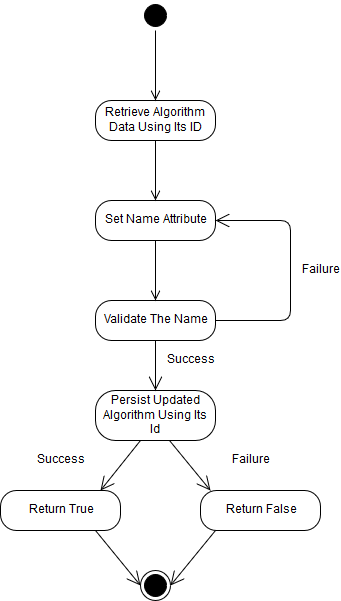
\includegraphics[width=12cm,height=15cm,keepaspectratio]{input_unit/images/update_algorithm_state_diagram.png}
    \begin{center}
    	\small{Figure 23: State diagram for updating an algorithm's name attribute }
    \end{center}
	\newpage
\subsection{Use Case diagram}
   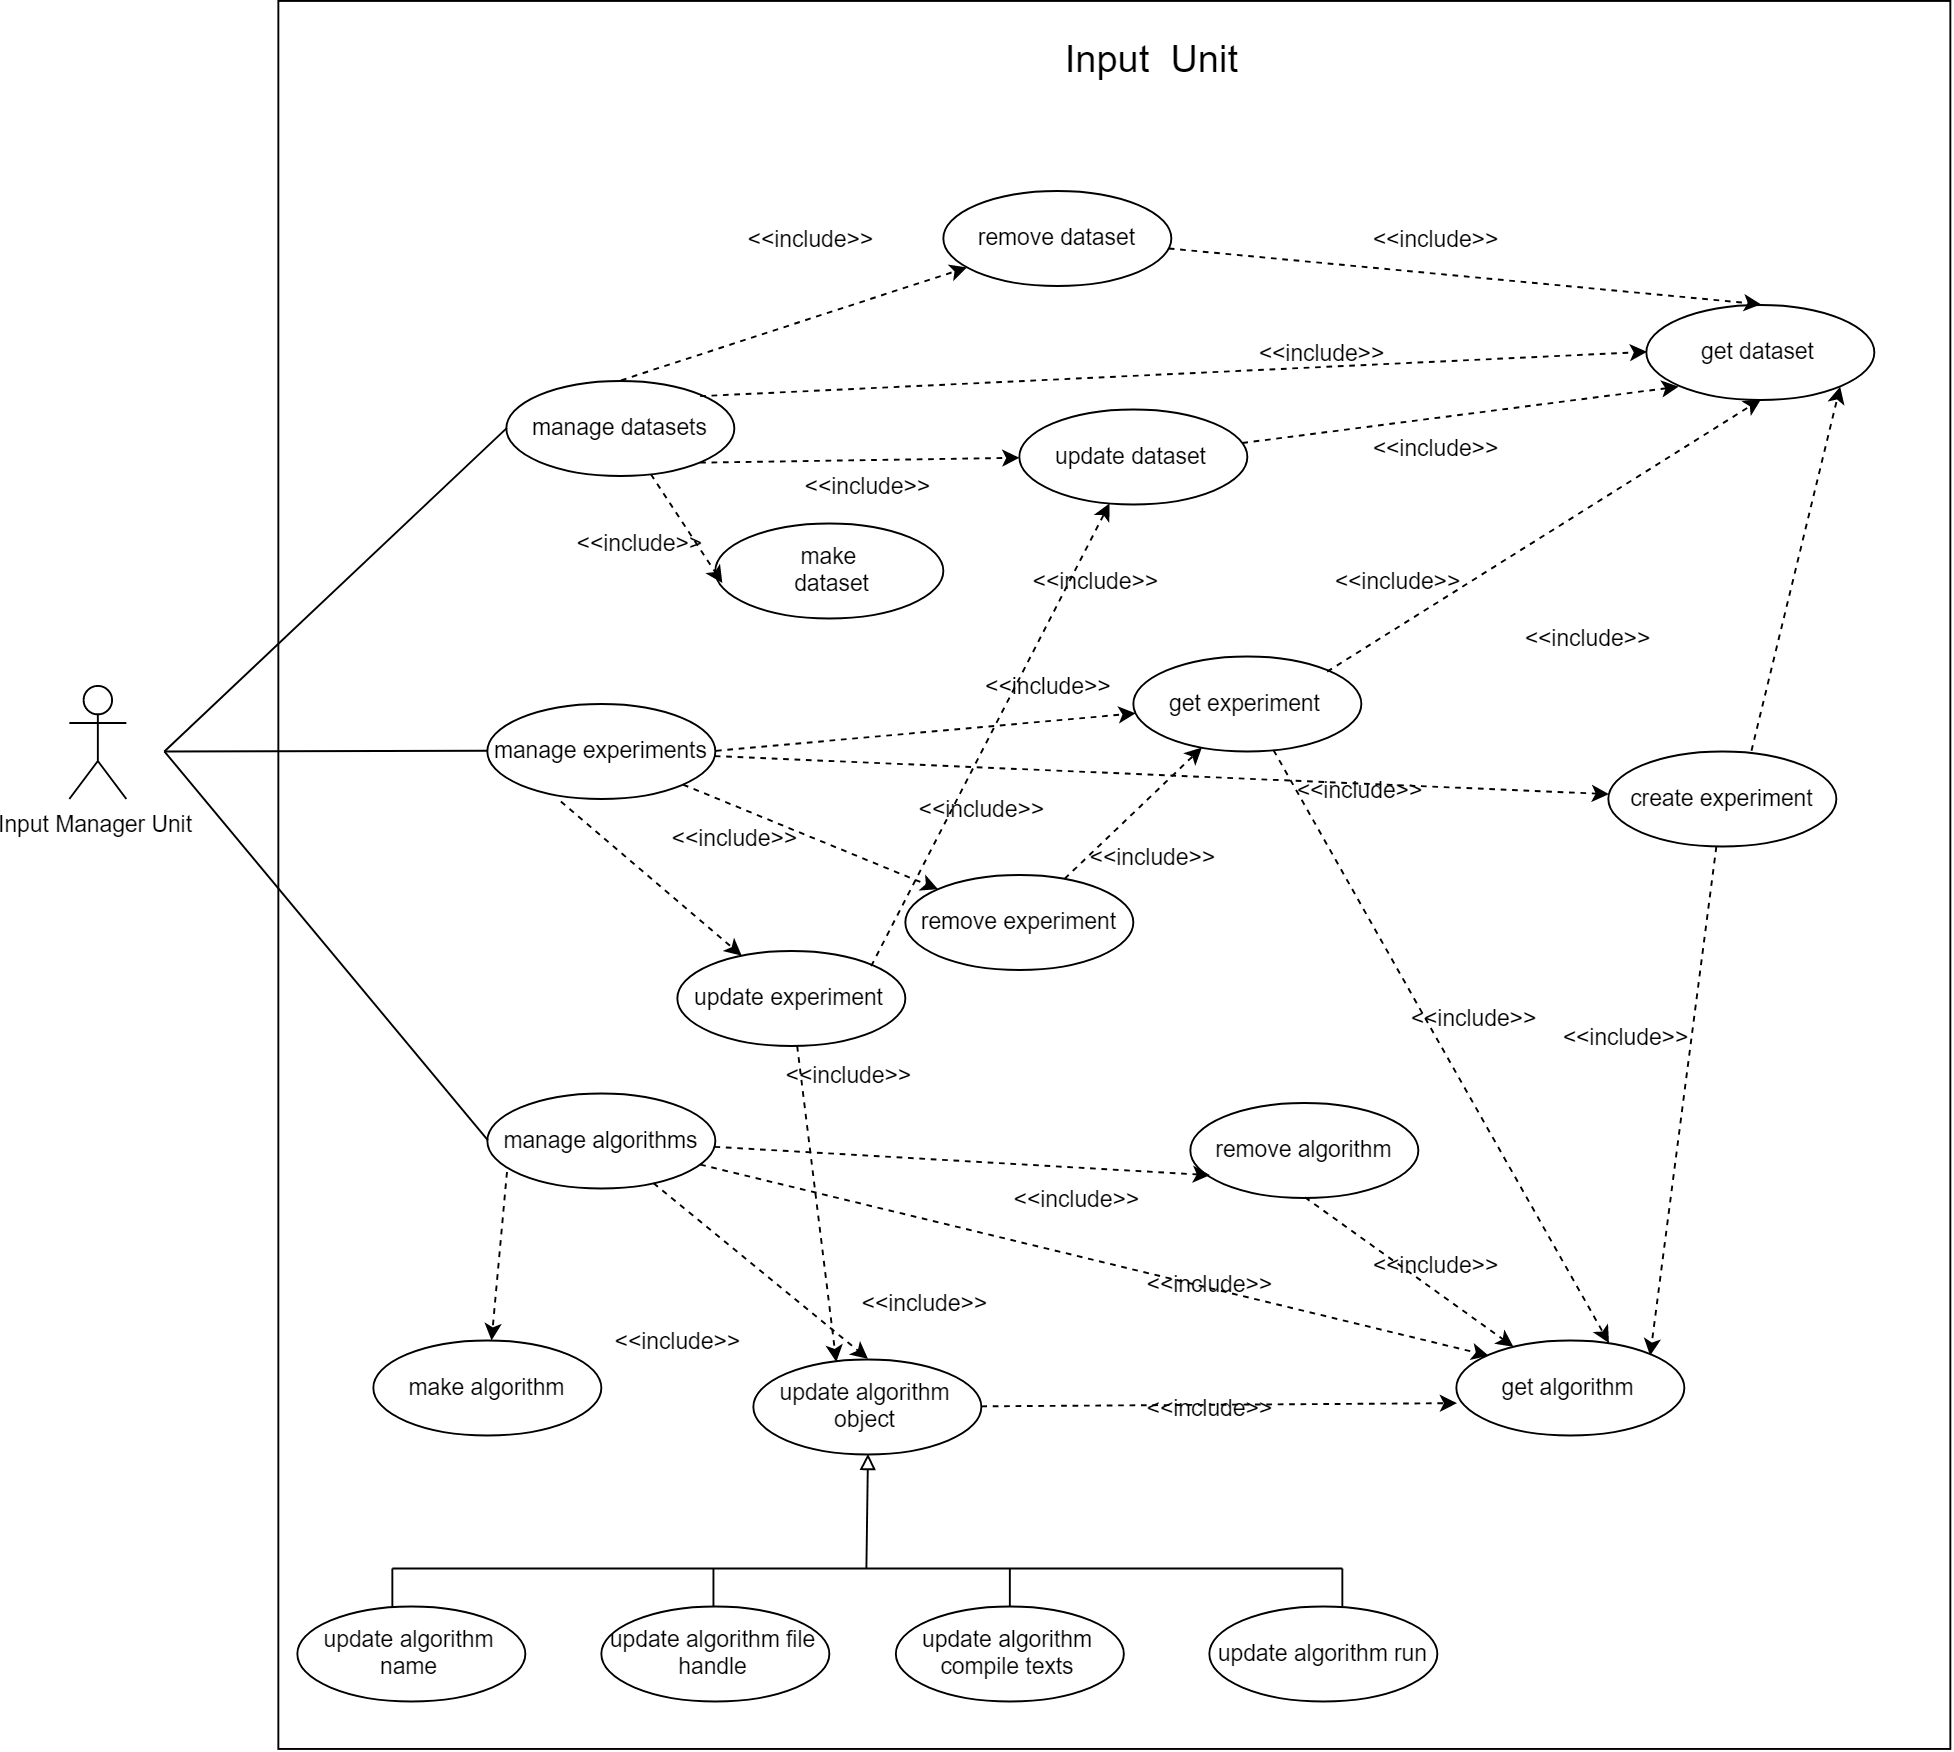
\includegraphics[width=12cm,height=15cm,keepaspectratio]{input_unit/images/input_unit_use_case.png}
    \begin{center}
    	\small{Figure 24: Use case diagram for Input Unit}
    \end{center}